
trie,有时称为前缀树,是一种搜索树,通常用于预测文本和其他搜索应用程序。trie是为深度优先搜索设计的递归结构,其中每个节点既是一个键,又是另一个trie。

一个常见的用例是字符串的trie,其中每个节点都是句子中的字符串。例如:

\begin{center}
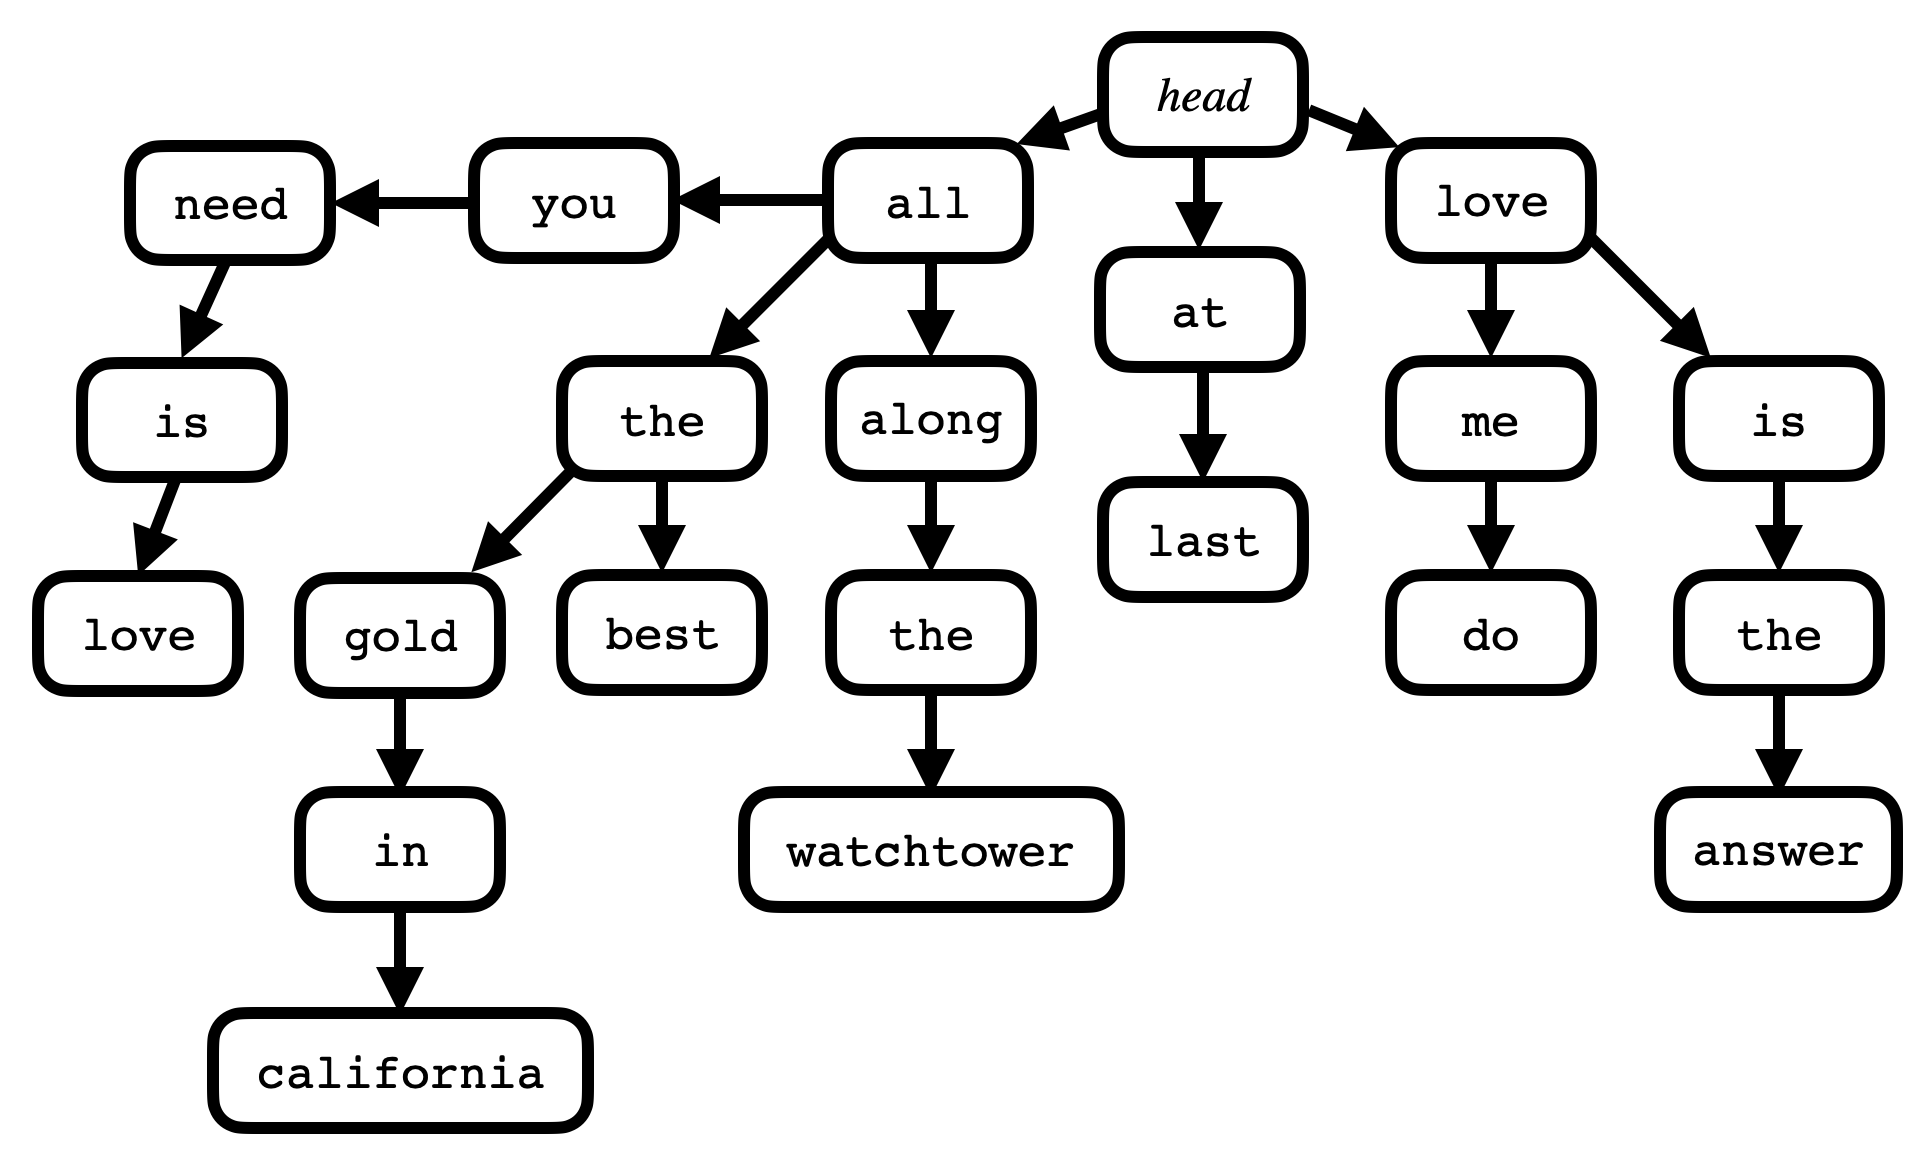
\includegraphics[width=0.8\textwidth]{content/chapter11/images/1.png}\\
图11.1 字符串trie
\end{center}

我们经常从树的头部开始搜索,寻找以特定单词开头的句子。在这个例子中,当我搜索all时,我得到了三个节点:you、the和along。

若寻找love,我得到的是me和is。

字符串trie通常用于创建搜索建议。这里,我们将使用std::map来实现一个字符串trie结构。

\subsubsection{How to do it…}

在这个示例中,创建了一个递归的trie类,将节点存储在std::map容器中。对于内存中的树来说,这是一个简单的解决方案。这是一个相当大的类,所以在这里只展示重要的部分。

要获得完整的类,请参阅源代码 \url{https://github.com/ PacktPublishing/CPP-20-STL-Cookbook/blob/main/chap11/trie.cpp}。

\begin{itemize}
\item 
起一个方便的别名:

\begin{lstlisting}[style=styleCXX]
using ilcstr = initializer_list<const char *>;
\end{lstlisting}

使用ilcstr来搜索trie。

\item 
把这个类放在一个私有命名空间中以避免冲突:

\begin{lstlisting}[style=styleCXX]
namespace bw {
	using std::map;
	using std::deque;
	using std::initializer_list;
\end{lstlisting}

方便起见,在这个命名空间中使用一些using语句。

\item 
类本身称为trie,其有三个数据成员:

\begin{lstlisting}[style=styleCXX]
class trie {
	using get_t = deque<deque<string>>;
	using nodes_t = map<string, trie>;
	using result_t = std::optional<const trie*>;
	
	nodes_t nodes{};
	mutable get_t result_dq{};
	mutable deque<string> prefix_dq{};
\end{lstlisting}

trie类有一些私有类型别名:

\begin{itemize}
\item 
get\_t是字符串的deque的deque,用于字符串结果。

\item 
nodes\_t是具有字符串键的trie类的map。

\item 
result\_t是指向trie指针的可选参数,用于返回搜索结果。空trie也是一个有效的结果,所以可以使用一个optional值。
\end{itemize}

nodes对象用于保存节点的递归map,其中trie上的每个节点都是另一个trie。

\item 
公共接口经常调用私有接口中的实用函数。例如,insert()方法接受一个initializer\_list对象,并调用私有函数\_insert():

\begin{lstlisting}[style=styleCXX]
void insert(const ilcstr& il) {
	_insert(il.begin(), il.end());
}
\end{lstlisting}

私有函数\_insert()执行插入元素的工作:

\begin{lstlisting}[style=styleCXX]
template <typename It>
void _insert(It it, It end_it) {
	if(it == end_it) return;
	nodes[*it]._insert(++it, end_it);
}
\end{lstlisting}

这方便了导航trie所需的递归函数调用。注意,引用一个不在map中出现的键,会创建一个带有该键的空元素。因此,若元素不存在,在nodes元素上使用\_insert()的那行代码,将创建空trie对象。

\item 
get()方法返回一个get\_t对象,我是字符串队列的队列的别名。这就可以返回多组结果:

\begin{lstlisting}[style=styleCXX]
get_t& get() const {
	result_dq.clear();
	deque<string> dq{};
	_get(dq, result_dq);
	return result_dq;
}
\end{lstlisting}

get()方法调用私有的\_get()函数,该函数递归遍历trie:

\begin{lstlisting}[style=styleCXX]
void _get(deque<string>& dq, get_t& r_dq) const {
	if(empty()) {
		r_dq.emplace_back(dq);
		dq.clear();
	}
	for(const auto& p : nodes) {
		dq.emplace_back(p.first);
		p.second._get(dq, r_dq);
	}
}
\end{lstlisting}

\item 
find\_prefix()函数的作用是:返回一个deque对象,其中包含与部分字符串的所有匹配项。

\begin{lstlisting}[style=styleCXX]
deque<string>& find_prefix(const char * s) const {
	_find_prefix(s, prefix_dq);
	return prefix_dq;
}
\end{lstlisting}

公共接口调用私有函数\_find\_prefix():

\begin{lstlisting}[style=styleCXX]
void _find_prefix(const string& s, auto& pre_dq) const {
	if(empty()) return;
	for(const auto& [k, v] : nodes) {
		if(k.starts_with(s)) {
			pre_dq.emplace_back(k);
			v._find_prefix(k, pre_dq);
		}
	}
}
\end{lstlisting}

私有\_find\_prefix()函数递归遍历trie,将前缀与每个键的开头进行比较。starts\_with()方法是C++20中的新方法。对于旧的STL,可以使用find()方法,并检查返回值是否为0:

\begin{lstlisting}[style=styleCXX]
if(k.find(s) == 0) {
	...
\end{lstlisting}

\item 
search()函数返回一个可选的<const trie*>,别名为result\_t。有两个重载:

\begin{lstlisting}[style=styleCXX]
result_t search(const ilcstr& il) const {
	return _search(il.begin(), il.end());
}
result_t search(const string& s) const {
	const ilcstr il{s.c_str()};
	return _search(il.begin(), il.end());
}
\end{lstlisting}

这些方法将迭代器传递给私有成员函数\_search(),该函数执行搜索工作:

\begin{lstlisting}[style=styleCXX]
template <typename It>
result_t _search(It it, It end_it) const {
	if(it == end_it) return {this};
	auto found_it = nodes.find(*it);
	if(found_it == nodes.end()) return {};
	return found_it->second._search(++it, end_it);
}
\end{lstlisting}

\_search()函数递归搜索,直到找到匹配项,然后返回result\_t对象中的节点。若没有找到匹配项,则返回非值optional值。

\item 
还有两个print\_trie\_prefix()函数的重载。这个函数从一个用作搜索键的前缀打印trie的内容。一个版本使用字符串作为前缀,另一个版本使用C-strings的initializer\_list:

\begin{lstlisting}[style=styleCXX]
void print_trie_prefix(const bw::trie& t,
		const string& prefix) {
	auto& trie_strings = t.get(\);
	cout << format("results for \"{}...\":\n", prefix);
	for(auto& dq : trie_strings) {
		cout << format("{} ", prefix);
		for(const auto& s : dq) cout << format("{} ", s);
		cout << '\n';
	}
}

void print_trie_prefix(const bw::trie& t,
		const ilcstr & prefix) {
	string sprefix{};
	for(const auto& s : prefix) sprefix +=
		format("{} ", s);
	print_trie_prefix(t, sprefix);
}
\end{lstlisting}

这些函数调用get()成员函数从trie中检索结果。

\item 
现在,可以在main()函数中测试trie类。首先,声明一个trie,并插入一些句子:

\begin{lstlisting}[style=styleCXX]
int main() {
	bw::trie ts;
	ts.insert({ "all", "along", "the", "watchtower" });
	ts.insert({ "all", "you", "need", "is", "love" });
	ts.insert({ "all", "shook", "up" });
	ts.insert({ "all", "the", "best" });
	ts.insert({ "all", "the", "gold", "in",
		"california" });
	ts.insert({ "at", "last" });
	ts.insert({ "love", "the", "one", "you're",
		"with" });
	ts.insert({ "love", "me", "do" });
	ts.insert({ "love", "is", "the", "answer" });
	ts.insert({ "loving", "you" });
	ts.insert({ "long", "tall", "sally" });
	...
\end{lstlisting}

insert()调用传递一个包含句子所有字符串的initializer\_list,句子的每个字符串都会插入到树的层次结构中。

\item 
现在,可以搜索这个trie。这里有一个简单的搜索单字符串“love”。

\begin{lstlisting}[style=styleCXX]
const auto prefix = {"love"};
if (auto st = ts.search(prefix); st.have_result) {
	print_trie_prefix(*st.t, prefix);
}
cout << '\n';
\end{lstlisting}

调用ts.search(),initializer\_list为一个C字串,称为prefix。结果连同前缀一起传递给print\_trie\_prefix()函数。

输出为:

\begin{tcblisting}{commandshell={}}
results for "love...":
love is the answer
love me do
love the one you're with
\end{tcblisting}

\item
下面是一个搜索双字符串前缀的例子:

\begin{lstlisting}[style=styleCXX]
const auto prefix = {"all", "the"};
if (auto st = ts.search(prefix); st.have_result) {
	print_trie_prefix(*st.t, prefix);
}
cout << '\n';
\end{lstlisting}

输出为:

\begin{tcblisting}{commandshell={}}
results for "all the ...":
all the best
all the gold in california
\end{tcblisting}

\item
下面是使用find\_prefix()函数搜索部分前缀:

\begin{lstlisting}[style=styleCXX]
const char * prefix{ "lo" };
auto prefix_dq = ts.find_prefix(prefix);
for(const auto& s : prefix_dq) {
	cout << format("match: {} -> {}\n", prefix, s);
	if (auto st = ts.search(s); st.have_result) {
		print_trie_prefix(*st.t, s);
	}
}
cout << '\n';
\end{lstlisting}

输出为:

\begin{tcblisting}{commandshell={}}
match: lo -> long
results for "long...":
long tall sally
match: lo -> love
results for "love...":
love is the answer
love me do
love the one you're with
match: lo -> loving
results for "loving...":
loving you
\end{tcblisting}

find\_prefix()搜索返回了几个结果,将每个结果传递给自己的搜索,每个结果产生几个结果。

\end{itemize}

\subsubsection{How it works…}

trie类的数据存储在递归map容器中。map中的每个节点都包含另一个trie对象,该对象又有自己的map节点。

\begin{lstlisting}[style=styleCXX]
using nodes_t = map<string, trie>
\end{lstlisting}

\_insert()函数接受begin和end迭代器,并使用它们在新节点上递归调用\_insert():

\begin{lstlisting}[style=styleCXX]
template <typename It>
void _insert(It it, It end_it) {
	if(it == end_it) return;
	nodes[*it]._insert(++it, end_it);
}
\end{lstlisting}

同样,\_search()函数在它找到的节点上递归调用\_search():

\begin{lstlisting}[style=styleCXX]
template <typename It>
result_t _search(It it, It end_it) const {
	if(it == end_it) return {this};
	auto found_it = nodes.find(*it);
	if(found_it == nodes.end()) return {};
	return found_it->second._search(++it, end_it);
}
\end{lstlisting}

这种使用std::map的递归方法可以有效地实现一个trie类。






























